\documentclass[tikz,border=7pt]{standalone}
% Shared TikZ style for the Nios V stereo accelerator diagrams.
\usepackage[T1]{fontenc}
\usepackage{lmodern}
\usepackage{xcolor}
\usepackage{tikz}
\usetikzlibrary{arrows.meta,backgrounds,calc,fit,positioning}

\definecolor{navy}{HTML}{073D73}
\definecolor{blue}{HTML}{0B5CAB}
\definecolor{cyan}{HTML}{1B8DBB}
\definecolor{green}{HTML}{27845B}
\definecolor{orange}{HTML}{C66A16}
\definecolor{red}{HTML}{B94444}
\definecolor{ink}{HTML}{172033}
\definecolor{muted}{HTML}{5A6678}
\definecolor{line}{HTML}{BFCBDA}
\definecolor{softblue}{HTML}{EDF4FA}
\definecolor{softcyan}{HTML}{ECF8FB}
\definecolor{softgreen}{HTML}{EEF8F2}
\definecolor{softorange}{HTML}{FFF4E8}
\definecolor{softgray}{HTML}{F5F7FA}

% Avoid automatic word hyphenation inside compact diagram nodes.
\hyphenpenalty=10000
\exhyphenpenalty=10000

\tikzset{
  font=\sffamily,
  block/.style={
    draw=line, rounded corners=2.2pt, fill=white,
    minimum height=10mm, text width=31mm, align=center,
    inner xsep=3mm, inner ysep=2.2mm
  },
  cpu/.style={block, draw=blue!55, fill=softblue},
  accel/.style={block, draw=cyan!65, fill=softcyan},
  memory/.style={block, draw=green!60, fill=softgreen},
  control/.style={block, draw=orange!65, fill=softorange},
  smallblock/.style={block, text width=24mm, minimum height=8mm, inner xsep=2mm, inner ysep=1.6mm},
  group/.style={draw=line, rounded corners=4pt, fill=softgray, inner sep=4mm},
  labeltag/.style={rounded corners=2pt, fill=navy, text=white, font=\sffamily\bfseries\footnotesize, inner xsep=2.5mm, inner ysep=1.2mm},
  flow/.style={-{Stealth[length=2.6mm,width=1.8mm]}, draw=navy, line width=0.85pt},
  dataflow/.style={-{Stealth[length=2.8mm,width=2mm]}, draw=blue, line width=1.15pt},
  controlflow/.style={-{Stealth[length=2.4mm,width=1.7mm]}, draw=orange, line width=0.9pt, dashed},
  returnflow/.style={-{Stealth[length=2.4mm,width=1.7mm]}, draw=green, line width=0.9pt},
  bus/.style={<->, >={Stealth[length=2.8mm,width=2mm]}, draw=navy, line width=1.6pt},
  note/.style={font=\sffamily\footnotesize, text=muted, align=left},
  arrowlabel/.style={font=\sffamily\scriptsize, text=muted, fill=white, inner sep=1.2pt}
}


\begin{document}
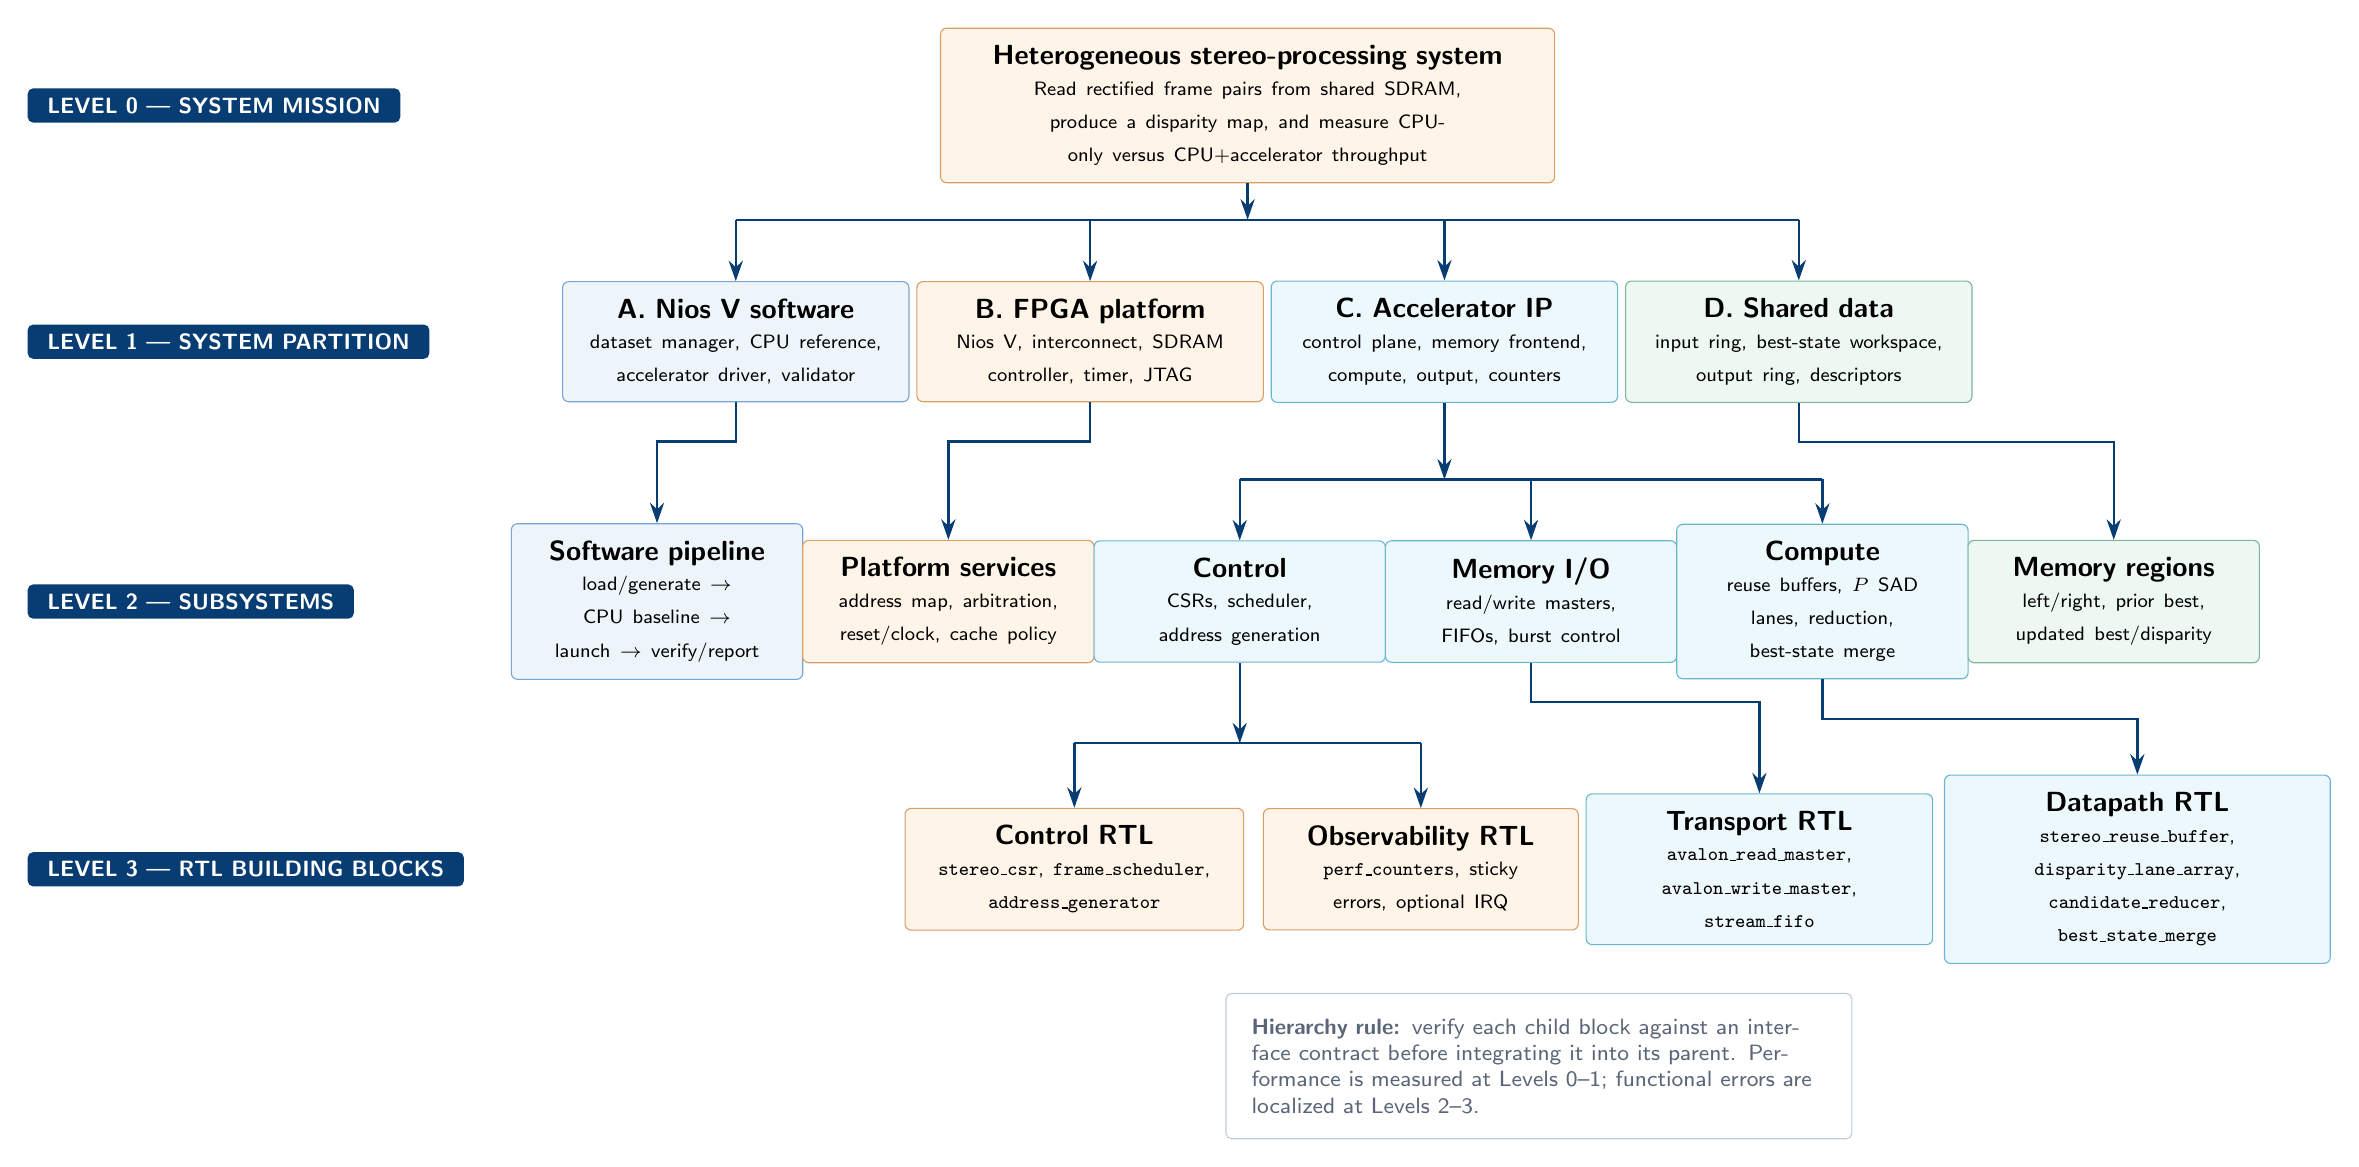
\begin{tikzpicture}[x=1cm,y=1cm]
  \node[labeltag, anchor=west] at (-4,0) {LEVEL 0 --- SYSTEM MISSION};
  \node[control, text width=72mm] (mission) at (11.5,0) {\textbf{Heterogeneous stereo-processing system}\\[-1pt]\scriptsize Read rectified frame pairs from shared SDRAM, produce a disparity map, and measure CPU-only versus CPU+accelerator throughput};

  \node[labeltag, anchor=west] at (-4,-3.0) {LEVEL 1 --- SYSTEM PARTITION};
  \node[cpu, text width=38mm] (sw) at (5.0,-3.0) {\textbf{A. Nios V software}\\[-1pt]\scriptsize dataset manager, CPU reference, accelerator driver, validator};
  \node[control, text width=38mm] (platform) at (9.5,-3.0) {\textbf{B. FPGA platform}\\[-1pt]\scriptsize Nios V, interconnect, SDRAM controller, timer, JTAG};
  \node[accel, text width=38mm] (accel) at (14.0,-3.0) {\textbf{C. Accelerator IP}\\[-1pt]\scriptsize control plane, memory frontend, compute, output, counters};
  \node[memory, text width=38mm] (memory) at (18.5,-3.0) {\textbf{D. Shared data}\\[-1pt]\scriptsize input ring, best-state workspace, output ring, descriptors};

  \draw[draw=navy, line width=.8pt] (5.0,-1.45) -- (18.5,-1.45);
  \draw[flow] (mission.south) -- (11.5,-1.45);
  \foreach \child in {sw,platform,accel,memory} {
    \draw[flow] (\child.north |- 0,-1.45) -- (\child.north);
  }

  \node[labeltag, anchor=west] at (-4,-6.3) {LEVEL 2 --- SUBSYSTEMS};
  \node[cpu, text width=31mm] (sw1) at (4.0,-6.3) {\textbf{Software pipeline}\\[-1pt]\scriptsize load/generate $\rightarrow$ CPU baseline $\rightarrow$ launch $\rightarrow$ verify/report};
  \node[control, text width=31mm] (pf1) at (7.7,-6.3) {\textbf{Platform services}\\[-1pt]\scriptsize address map, arbitration, reset/clock, cache policy};
  \node[accel, text width=31mm] (ac1) at (11.4,-6.3) {\textbf{Control}\\[-1pt]\scriptsize CSRs, scheduler, address generation};
  \node[accel, text width=31mm] (ac2) at (15.1,-6.3) {\textbf{Memory I/O}\\[-1pt]\scriptsize read/write masters, FIFOs, burst control};
  \node[accel, text width=31mm] (ac3) at (18.8,-6.3) {\textbf{Compute}\\[-1pt]\scriptsize reuse buffers, $P$ SAD lanes, reduction, best-state merge};
  \node[memory, text width=31mm] (mem1) at (22.5,-6.3) {\textbf{Memory regions}\\[-1pt]\scriptsize left/right, prior best, updated best/disparity};

  \draw[flow] (sw.south) -- ++(0,-5mm) -| (sw1.north);
  \draw[flow] (platform.south) -- ++(0,-5mm) -| (pf1.north);
  \draw[draw=navy, line width=.8pt] (ac1.north |- 0,-4.75) -- (ac3.north |- 0,-4.75);
  \draw[flow] (accel.south) -- (accel.south |- 0,-4.75);
  \foreach \child in {ac1,ac2,ac3} {
    \draw[flow] (\child.north |- 0,-4.75) -- (\child.north);
  }
  \draw[flow] (memory.south) -- ++(0,-5mm) -| (mem1.north);

  \node[labeltag, anchor=west] at (-4,-9.7) {LEVEL 3 --- RTL BUILDING BLOCKS};
  \node[control, text width=37mm] (r0) at (9.3,-9.7) {\textbf{Control RTL}\\[-1pt]\scriptsize \texttt{stereo\_csr}, \texttt{frame\_scheduler}, \texttt{address\_generator}};
  \node[control, text width=34mm] (r3) at (13.7,-9.7) {\textbf{Observability RTL}\\[-1pt]\scriptsize \texttt{perf\_counters}, sticky errors, optional IRQ};
  \node[accel, text width=38mm] (r1) at (18.0,-9.7) {\textbf{Transport RTL}\\[-1pt]\scriptsize \texttt{avalon\_read\_master}, \texttt{avalon\_write\_master}, \texttt{stream\_fifo}};
  \node[accel, text width=43mm] (r2) at (22.8,-9.7) {\textbf{Datapath RTL}\\[-1pt]\scriptsize \texttt{stereo\_reuse\_buffer}, \texttt{disparity\_lane\_array}, \texttt{candidate\_reducer}, \texttt{best\_state\_merge}};

  \draw[draw=navy, line width=.8pt] (r0.north |- 0,-8.1) -- (r3.north |- 0,-8.1);
  \draw[flow] (ac1.south) -- (ac1.south |- 0,-8.1);
  \draw[flow] (r0.north |- 0,-8.1) -- (r0.north);
  \draw[flow] (r3.north |- 0,-8.1) -- (r3.north);
  \draw[flow] (ac2.south) -- ++(0,-5mm) -| (r1.north);
  \draw[flow] (ac3.south) -- ++(0,-5mm) -| (r2.north);

  \node[note, text width=73mm] (rule) at (15.2,-12.2) {\textbf{Hierarchy rule:} verify each child block against an interface contract before integrating it into its parent. Performance is measured at Levels 0--1; functional errors are localized at Levels 2--3.};
  \draw[draw=line, rounded corners=2pt] ([xshift=-2mm,yshift=-2mm]rule.south west) rectangle ([xshift=2mm,yshift=2mm]rule.north east);
\end{tikzpicture}
\end{document}
